\documentclass[11pt]{article}
\usepackage{amsmath,textcomp,amssymb,geometry,graphicx,float,mathrsfs,tabularx}

\def\Login{ee121-af} % Your login
\def\HW{3} % Homework number

\title{EE 121 -- Fall 2013\\Homework 2}

\markboth{EE 121 -- Fall 2013 Homework \HW}{EE 121 -- Fall 2013 Homework \HW}
\pagestyle{myheadings}

\begin{document}
\maketitle
\noindent\textbf{Team Bitdiddlers} \\
\text{Jeff Lievense, Rishi Sharma, Nader Behdin, Tim Brown}

\begin{enumerate}
  % Have a new \item for each problem
  % Make sure you have a \newpage after each item


  % PROBLEM 1
  \item
    \begin{enumerate}


        %part a)
        \item We generate a generator matrix row by row by creating a random bit string (length $k$) of Bernoulli Random Variables ($\mathcal{B}(\frac{1}{2})$) and appending them to our matrix $G$. The dot product of each row with the message (mod 2) is the parity bit for each row. We can decode when our generator matrix is full rank (i.e. we can solve a system of k equations), and the following plot shows an estimate of the PMF (generated by a normalized histogram) of $N$, number of rows necessary to decode a message of length $k=10$ and $k=100$ in 100 trials.



        % part b)
        \item Now we generate rows of a generator matrix $G$ in the same fashion as before, but they are drawn from the ideal and robust soliton distribution.



        % part c)
        \item





        % part d)
        \item




    \end{enumerate}
    \newpage




% PROBLEM 2
  \item
    \begin{enumerate}

        % part a)
        \item


        % part b)
        \item
            Let $\vec{m}$ be a $k = \alpha s$ bit message that we'd like to send over an unreliable erasure channel (BEC with bit-erasure probability $p$) without any coding, and assume we can send $\vec{r} = H\vec{m}$, the $s$-bit parity of $\vec{m}$, over a reliable channel (i.e. the receiver knows $\vec{r}$). The receiver also gets $\vec{y}$, which is the result of sending $\vec{m}$ over the BEC. Since all non-erased bits are correct, for each $y_i$ that is not erased, we have $y_i = m_i$. Our scheme works as follows:
            \begin{itemize}
                \item Compute $H\vec{y}$ and replace each erasure with some variable $e_i$.
                \item Were there no erasures, we would have $H\vec{y} = H\vec{m} = \vec{r}$. So, we set $H\vec{y} = \vec{r}$, yielding the following system of equations,
                    \begin{flalign*}
                        h_{11}y_1 + \dotsc + h_{1k}y_k &= r_1 \\
                        &\vdots \\
                        h_{s1}y_1 + \dotsc + h_{sk}y_k &= r_s
                    \end{flalign*}
                    where some number of the $y_i$s will be replaced with $e_i$s.
                \item Solve for all $e_i$s and reconstruct $\vec{m}$.
            \end{itemize}
            The Law of Large Numbers tells us we should expect roughly $k(p + \epsilon)$ erasures, so we decode only when less than $k(p + \epsilon)$ erasures occur, otherwise we declare error. If there aren't too many erasures, error occurs if any false message's syndrome (parity bits) matches the received message $\vec{y}$'s syndrome ($H\vec{y}$, with erasures) -- this occurs when a false message matches the received message (with erasures). We can compute the probability of error as follows:
            \begin{flalign*}
                P(\mbox{error}) &= P(\mbox{at least one false syndrome matches received syndrome}) \\
                &\leq 2^s\cdot2^{-k(p + \epsilon)} \\
                &= 2^{s - k(p + \epsilon)} \\
                &= 2^{s(1 - \alpha(p + \epsilon))}
            \end{flalign*}
            The inequality comes from a union bound -- there are $2^s$ possible syndromes, and the probability of any one false syndrome matching the received syndrome is equal to the probability that all of the non-erased message bits match a false message. There are $2^k$ total messages, and if we only decode when there are $k(1 - (p + \epsilon))$ non-erased bits, there are $2^{k(1 - (p + \epsilon))}$ messages that could match the received message with erasures. Then the probability of one false syndrome matching the received syndrome is simply $\frac{2^{k(1 - (p + \epsilon))}}{2^k} = 2^{-k(p + \epsilon)}$. \\
            \\
            We then choose the "reliability amplification" parameter $\alpha$ such that the probability of error goes to zero with $s$, i.e. the exponent in the probability of error must be negative:
            \begin{flalign*}
                1 - \alpha(p + \epsilon) &< 0 \\
                \alpha &> \frac{1}{p + \epsilon}
            \end{flalign*}
            And thus we see that, if we choose $\alpha > \frac{1}{p}$, this scheme will work with probability of error going to zero with $s$.

        % part c)
        \item
            Consider a message $\vec{m}$ of length $n = \alpha k = \alpha^2 s$. We would like to send this message over an unreliable channel without any coding. Let $H_1$ be a dense random parity-check matrix that linearly maps $n = \alpha k$ bits into $k$ parities. In parts a) and b), we showed that we can recover $\alpha s$ unreliable bits from $s$ reliable bits. So, if we can reliably send the $k$ parity bits computed via $H_1\vec{m}$, we can use them to recover the $n = \alpha k$ bits of $\vec{m}$. How do we reliably send the $k$ parity bits of $H_1\vec{m}$? We use the same strategy: let $H_2$ be a different dense random parity-check matrix that linearly maps $k = \alpha s$ bits into $s$ parities. We can then recover the $k = \alpha s$ bits of $H_1\vec{m}$ from the $s$ parity bits computed via $H_2(H_1\vec{m})$, since we can send $s$ bits reliably. Thus, if we can reliably send the $s$ bits of $H_2(H_1\vec{m})$, we can use them to recover the $k = \alpha s$ bits of $H_1\vec{m}$, which we can use to recover the $n = \alpha k = \alpha^2 s$ bits of $\vec{m}$.

        % part d)
        \item

        \begin{itemize}
            \item
                {\bf Binary Symmetric Channel} \\
                \\
                Let $\vec{t}$ be the $s$ bit message we're trying to communicate. We want to use a $\frac{1}{R}$-repetition code to encode $\vec{t}$ as $\vec{u}$, an $\frac{s}{R}$ bit codeword made up of $s$ blocks, each containing $\frac{1}{R}$ bits. We then send $\vec{u}$ over a BSC with bit-error probability $p$. Call the received codeword (with errors) $\vec{v}$. We decode $\vec{v}$ to the $s$ big message $\hat{t}$ via majority decoding:
                \begin{itemize}
                    \item
                        For the $i^{\mbox{th}}$ block of $\vec{v}$:
                            \begin{itemize}
                                \item
                                    If there are more ones than zeros, decode the $i^{\mbox{th}}$ bit of $\hat{t}$ as one, and vice versa.
                            \end{itemize}
                \end{itemize}
                In this scheme, an error occurs if at least half of the bits in at least one block are corrupt. For a single block, let $X_i$ be an indicator random variable on the $i^{\mbox{th}}$ bit in the block being corrupt ($X_i\sim\mathcal{B}(p)$, i.i.d. over $i$), and let $Y = \sum_{i = 1}^{\frac{1}{R}}$. Then:
                \begin{flalign*}
                    P(\mbox{at least half of one block is corrupt}) &= P(Y \geq \frac{1}{2}\cdot\frac{1}{R}) \\
                    &\leq \underset{t > 0}{\mbox{min}} \frac{\prod_{i = 1}^{\frac{1}{R}}\mathbb{E}[e^{tX_i}]}{e^{\frac{t}{2R}}}
                \end{flalign*}
                The above inequality is the result of a Chernoff bound. It can be shown that, for a sum of i.i.d. $\mathcal{B}(p)$ random variables, the minimizing $t$ is $\log{\frac{1 - p}{p}}$. Substituting this value yields:
                \begin{flalign*}
                    P(\mbox{block error}) &\leq (2(p(1 - p))^{\frac{1}{2}})^{\frac{1}{R}} \\
                    P(\mbox{error}) &= P(\mbox{at least one block error}) \leq s\cdot(2(p(1 - p))^{\frac{1}{2}})^{\frac{1}{R}}
                \end{flalign*}
                The last equality is the result of a union bound -- all bit-erasures are independent, so all block-erasures are independent. If we are willing to tolerate $P(\mbox{error}) \leq \delta$, then:
                \begin{flalign*}
                    P(\mbox{error}) \leq s\cdot(2(p(1 - p))^{\frac{1}{2}})^{\frac{1}{R}} &\leq \delta \\
                    \frac{1}{R}\log{(2(p(1-p))^{\frac{1}{2}})} \leq \log{\frac{\delta}{s}} \\
                    \frac{1}{R} \geq \frac{\log{\frac{\delta}{s}}}{\log{(2(p(1 - p))^{\frac{1}{2}})}}
                \end{flalign*}
                Thus, if we repeat each bit of $\vec{t}$ at least $\frac{\log{\frac{\delta}{s}}}{\log{(2(p(1 - p))^{\frac{1}{2}})}}$ times, we will successfully communicate $\vec{t}$ with probability $1 - \delta$. The rate of this code is then $R \leq \frac{\log{(2(p(1 - p))^{\frac{1}{2}})}}{\log{\frac{\delta}{s}}}$

            \item
                {\bf Binary Erasure Channel} \\
                \\
                Let $\vec{t}$ be the $s$ bit message we're trying to communicate. We want to use a $\frac{1}{R}$-repetition code to encode $\vec{t}$ as $\vec{u}$, an $\frac{s}{R}$ bit codeword made up of $s$ blocks, each containing $\frac{1}{R}$ bits. We then send $\vec{u}$ over a BEC with bit-erasure probability $p$. Call the received codeword (with erasures) $\vec{v}$. Since all non-erased bits are correct, we decode $\vec{v}$ to the $s$ bit message $\hat{t}$ via the following strategy:
                \begin{itemize}
                    \item
                        For the $i^{\mbox{th}}$ block of $\vec{v}$:
                            \begin{itemize}
                                \item
                                    If not all bits are erased, decode bit $i$ of $\hat{t}$ as the non-erased bits of block $i$.
                            \end{itemize}
                \end{itemize}
                In this scheme, an error occurs if at least one block has all $\frac{1}{R}$ bits erased.
                \begin{flalign*}
                P(\mbox{all bits in one block erased}) &= p^{\frac{1}{R}} \\
                P(\mbox{error}) &= P(\mbox{all bits in at least one block erased}) \leq s\cdot p^{\frac{1}{R}}
                \end{flalign*}
                The last equality is the result of a union bound -- all bit-erasures are independent, so all block-erasures are independent. If we are willing to tolerate $P(\mbox{error}) \leq \delta$, then:
                \begin{flalign*}
                    P(\mbox{error}) \leq s\cdot p^{\frac{1}{R}} &\leq \delta \\
                    p^{\frac{1}{R}} &\leq \frac{\delta}{s} \\
                    \log{p^{\frac{1}{R}}} \leq \log{\frac{\delta}{s}} \\
                    \frac{1}{R}\log{p} \leq \log{\frac{\delta}{s}} \\
                    \frac{1}{R} \geq \frac{\log{\frac{\delta}{s}}}{\log{p}}
                \end{flalign*}
                Thus, if we repeat each bit of $\vec{t}$ at least $\frac{\log{\frac{\delta}{s}}}{\log{p}}$ times, we will successfully communicate $\vec{t}$ with probability $1 - \delta$. The rate of this code is then $R \leq \frac{\log{p}}{\log{\frac{\delta}{s}}}$
        \end{itemize}



        % part e)
        \item

        \begin{itemize}
            \item
                {\bf Binary Symmetric Channel}

            \item
                {\bf Binary Erasure Channel}

        \end{itemize}


        %part f)
        \item



        %part g)
        \item
            If we use a parity matrix $H$ with exactly three ones in each column and exactly thirty ones in each row, this means the bipartite graph representation has $3k$ edges going from the $k$ data bits to the $s$ parity bits and $30s$ edges going from the $s$ parity bits to the $k$ data bits. Both numbers must be the same, so we set them equal to each other and solve:
            \begin{flalign*}
                30s = 3k \\
                s = \frac{k}{10}
            \end{flalign*}
            So, for $k$ data bits, there are $\frac{k}{10}$ parity bits, and the size of $H$ is $\frac{k}{10} \times k$ (rows $\times$ columns).


        %part h)
        \item
            We will find the probability that a loop exists in the first level of the tree by drawing a parallel between this problem and the Birthday Paradox. There are $k$ total data bits in the tree, and there are 88 data bits in the first level. A cycle exists if any data bit shows up more than once in the first level. Let us look at the total number of data bits $k$ as the total number of possible birthdays, and the 88 data bits as the number of people in a room. The probability of a loop existing is the complement of the probability that no loop exists, which is equivalent to the probability that no data bit shows up more than once, which is equivalent to no two people of the 88 people in a room having the same birthday. This probability is:
            \begin{flalign*}
                P(\mbox{no two people have the same birthday}) &= \frac{k\mbox{P}88}{k^{88}} \\
                &= \frac{k!}{(k - 88)!k^{88}} \\
                &= \frac{(k - 0)(k - 1)\cdots(k - 87)}{k^{88}} \\
                &= \frac{k^{88}}{k^{88}}(1 - \frac{0}{k})(1 - \frac{1}{k})\dotsc(1 - \frac{86}{k}) \\
                &\approx 1 - e^{-\frac{0}{k}}e^{-\frac{1}{k}}\dotsc e^{-\frac{87}{k}} \\
                &= e^{-\frac{1}{k}\sum_{i = 1}^{87}} \\
                &= e^{-\frac{87\cdot86}{2k}}
            \end{flalign*}
            The probability of a loop existing in the first level is simply the complement of the above probability, and we want to bound that by $\delta$:
            \begin{flalign*}
                1 - e^{-\frac{87\cdot86}{2k}} &\leq \delta \\
                e^{-\frac{87\cdot86}{2k}} &\geq 1 - \delta \\
                -\frac{87\cdot86}{2k} &\geq \log{1 - \delta} \\
                k &\geq \frac{87\cdot86}{\log{\frac{1}{1 - \delta}}}
            \end{flalign*}
            Thus, if we are willing to tolerate a loop probability of $\delta$, $k$ must be larger than $\frac{87\cdot86}{\log{\frac{1}{1 - \delta}}}$.
            
            
        % part i)
        \item
            

        % part j)
        \item


        % part k)
        \item
            From the plot, we see that, for $p = 0.05$, the path taken by the probability of error on a bit as we move up the tree towards the root converges to zero:
        \begin{figure}[H]
            \begin{center}
                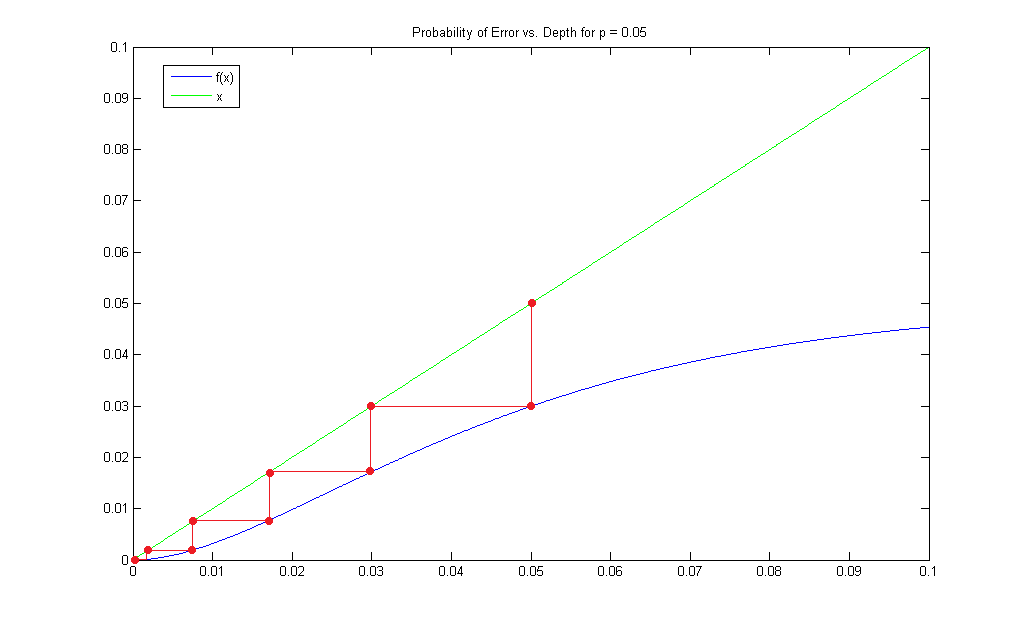
\includegraphics[width = \textwidth]{figure_k.png}
                \caption{}
            \end{center}
        \end{figure}


        % part l)
        \item


        % part m)
        \item

        % part n)
        \item
            By increasing $p$ and re-plotting until $f(x)$ intersects the function $x$, we see that the decoding method will fail roughly around $p \geq 0.083$:
        \begin{figure}[H]
            \begin{center}
                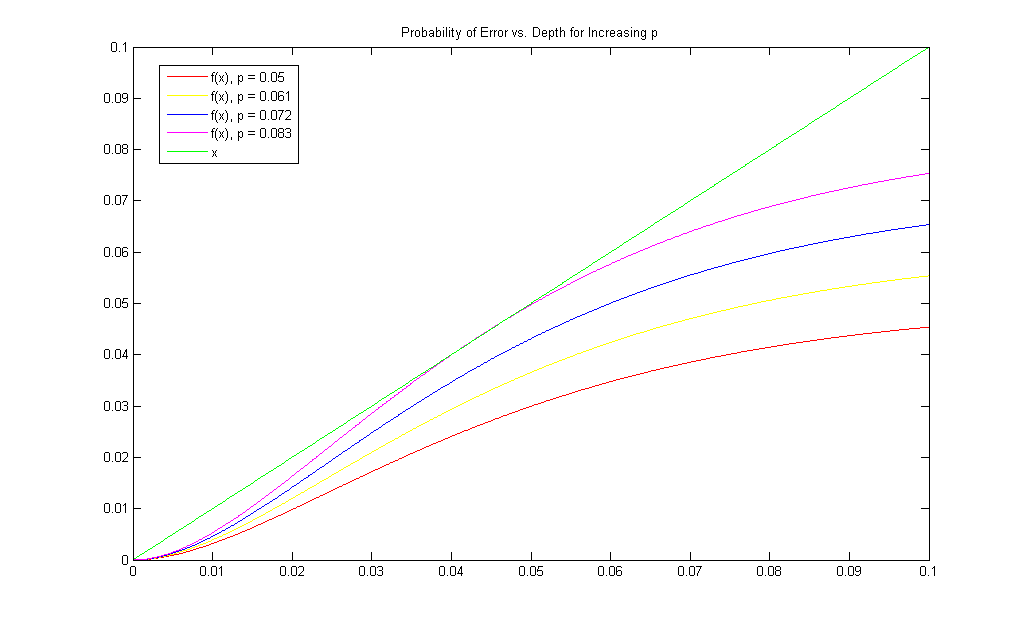
\includegraphics[width = \textwidth]{figure_n.png}
                \caption{}
            \end{center}
        \end{figure}
            \noindent
        % part o)
        \item
            From the plot in the previous part, we see that, from about $p = 0.03$ to $p = 0.05$, $f(x)$ is very close to the function $x$. This means the path taken by the probability of error has a lot more "turns" than it would for lower values of $p$. In other words, since $f(x)$ and the function $x$ are very close for values of $p$ close to the threshold value, the path "bounces" back \& forth very rapidly, which means the decoding process will take many, many more iterations.


        % part p)
        \item




    \end{enumerate}
    \newpage



  % PROBLEM 3
  \item

    \newpage

\end{enumerate}
\end{document} 